\documentclass{article}


\usepackage{minted}
\usepackage{fancyhdr}
\usepackage{amsmath,amssymb,amsthm}
\usepackage{graphicx}
\usepackage{pdfpages}
\usepackage[margin=1in]{geometry}
\usepackage{parskip}
\usepackage{caption}
\usepackage{listings}
\usepackage{physics}
\usepackage{mathtools}
\usepackage{xparse}
\usepackage{dsfont}
\usepackage{amsmath}
\usepackage{amssymb}


\title{	
	\normalfont\normalsize
	\vspace{25pt} % Whitespace
	\rule{\linewidth}{0.5pt}\\ % Thin top horizontal rule
	\vspace{20pt} % Whitespace
	{\huge MATH240 Assignment 2 - Real Analysis}\\ % The assignment title
	\vspace{12pt} % Whitespace
	\rule{\linewidth}{2pt}\\ % Thick bottom horizontal rule
	\vspace{12pt} % Whitespace
}

\author{\LARGE Emma Hogan \\\\53837798} % Your name


\date{\normalsize\today} % Today's date (\today) or a custom date
\begin{document}
\begin{titlepage}
\maketitle
\thispagestyle{empty}
\begin{figure}[!htb]
\centering
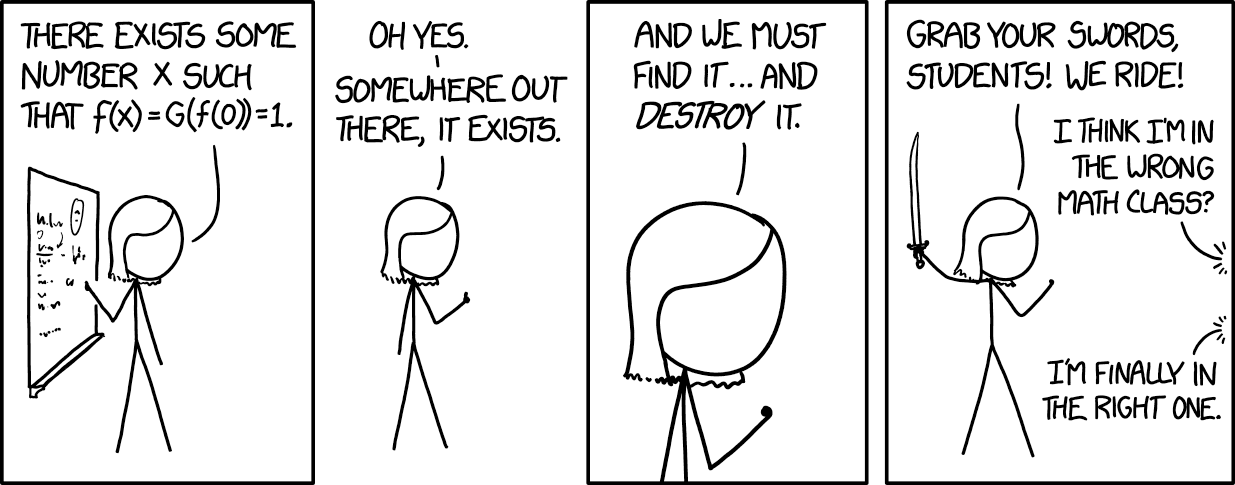
\includegraphics[width=\textwidth]{xkcd.png}
\caption*{xkcd 1856: Existence Proof}
\end{figure}
\end{titlepage}
\section*{Question 1}
\subsection*{Let S be a non-empty subset of the real numbers which is bounded above. Let c be a real number and define T = \{cx $\mid$ x $\in$ S\}. Show that, if c $>$ 0, then T is non empty, bounded above and that supT = csupS. Give an example of a set S as above, such that, with c = -1, the set T is still bounded above but supT $\ne$ csupS.}

\solution
To show \(T\) is non-empty, observe \(S\) \(\neq \emptyset\), so \(T = \{cx\) \(|\) \(x \in S\} \neq \emptyset\).
\\
\\
Since \(S\) is bounded above, by definition there exists some upper bound \(U\) such that \(x \leq U\) \(\forall\) \(x \in S\). So, since \(c\) is positive, \(cx \leq cU\) \(\forall\) \(x \in S\). Therefore, \(cU\) is an upper bound for \(T\).
\\
\\
Since \(S\) is non-empty and bounded above, we know \(supS\) exists. By definition of \(supS\), this is an upper bound for S, so from our previous result, we know \(csupS\) is an upper bound for T. That is, \(t \leq csupS\) \(\forall\) \(t \in T\).
\\
\\
Since \(T\) is also non-empty and bounded above, we know \(supT\) also exists. Assume \(supT < csupS\). We will find a contradiction.
\\
\\
Since \(c > 0\):
\begin{align}
  \label{}
  supT < csupS \nonumber \\
  \Rightarrow \frac{supT}{c} < supS\nonumber
\end{align}
\\
By definition of \(supS\), for any value \(X < supS\), \(\exists\) \(s \in S\) such that \(s>X\). So, \(\exists\) \(s' \in S\) such that
\begin{align}
  \label{}
  s' > \frac{supT}{c} \nonumber \\
  \Rightarrow cs' > supT \nonumber
\end{align}
\\
\(cs' \in T\) by definition of \(T\), so \(cs' > supT\) is a contradiction.
\\
\begin{align}
  \label{}
  \therefore supT \geq csupS
\end{align}
\\
But \(csupS\) is an upper bound for \(T\).
\begin{align}
  \label{}
  \therefore supT \leq csupS
\end{align}
\\
And so from (1) and (2), we know:
\begin{align}
  \label{}
  supT = csupS \nonumber
\end{align}
\\
As an example of \(supT \neq supS\) when \(c=-1\), take \(S = \{-1,-2\}\), so \(supS = -1\). With \(c=-1\), \(T = \{1,2\}\) and \(supT = 2\). But \(csupS = 1 \neq 2\), so \(csupS \neq supT\).
\\\\\\
\section*{Question 2}
\subsection*{(i) If (\(x_n\)) is a sequence such that lim\(|x_n|\) = 0, prove that lim\(x_n\) = 0 also.}

\solution
\\
By definition of the limit, \(\lim|x_n| = 0 \Rightarrow \forall\) \(\mathcal{E} \geq 0\), \(\exists\) \(N \in \mathds{N}\) such that \(\forall\) \(n\) \(\geq N\), \(||x_n| - 0| \leq \matthcal{E}\).
\begin{align}
  \label{}
  ||x_n| - 0| \leq \mathcal{E} \nonumber \\
  \Rightarrow ||x_n|| \leq \mathcal{E} \nonumber \\
  \Rightarrow |x_n| \leq \mathcal{E} \nonumber \\
  \Rightarrow |x_n - 0| \leq \mathcal{E} \nonumber \\
  \Rightarrow \lim x_n = 0 \nonumber
\end{align}

\subsection*{(ii) Give an example of a sequence \((x_n)\) that does not converge but that (\(|x_n|\)) converges.}
\solution
\\
Define \((x_n)\) by \(x_n\ = (-1)^n\) which does not converge.
\\
\\
\(|x_n| = |(-1)^n| = |-1|^n = 1\) so \((|x_n|)\) converges to 1.
\\\\\\
\section*{Question 3}
\subsection*{Let $\sum x_n$ be a series that converges absolutely. Show that $\sum x^2_n$ converges.}
\solution
\\
\\
\\
Since \(\sum |x_n|\) converges, we know that $\lim_{n\to\infty} |x_n|$\(=0\). So, by definition of the limit, we know \(\exists\) \(N\) such that \(\forall\) \(n\) \(\geq N\), \(|x_n| \leq 1\).
\\
\\
We can remove a finite number of terms for the start of a series without changing its behaviour. So, we consider \(\sum_{n=N}^{\infty} |x_n|\), so \(|x_n|\leq 1\) for every term in the sequence.
\\
\\
Note that since \(x_n^2 \geq 0\), \(|x_n|^2 = x_n^2 = |x_n^2|\). 
\\
\\
\(|x_n| \leq 1\) so \(|x_n|^2 = |x_n^2| \leq 1\).
\\
\\
\(|x_n^2| \leq |x_n|\) \(\forall n \geq N\), so, since \(\sum_{n=N}^{\infty} |x_n|\) is convergent, \(\sum_{n=N}^{\infty} |x_n^2|\) is also convergent. Once again, N is just a finite number so removing the first N terms has not changed the behaviour of the series.
\\
\\
Therefore \(\sum x_n^2\) is absolutely convergent, which implies it is convergent.
\\
\\
\\
\section*{Question 4}
\subsection*{Prove, from the definition of limit, that \lim_{n\to\infty} x^2+x$ = 2.}
\solution
\\\\
The limit definition states:
\\
\(lim_{x\to p} f(x) = L\) \(\Rightarrow\) \(\forall\) \(\mathcal{E} > 0\), \(\exists\) \(\delta > 0\) such that, \(\forall x \in \mathds{R}\), \(0 < |x-p| < \delta\) we have \(x\) in the domain of \(f\) and \(|f(x)-L| < \mathcal{E}\).
\\
\\
So, to show \(lim_{x\to p} (x^2 + x - 2)\), we need to find \(\delta > 0\) such that, \(\forall\) \(x \in \mathds{R}\), \(0<|x-1|<\delta\), we have \(|x^2+x-2| < \mathcal{E}\) \(\forall\) \(\mathcal{E}\).
\\
\\
Choose \(\delta = min\left\{\frac{\mathcal{E}}{4},1\right\}\).
\\
\begin{align*}
  |x^2 + x - 2| &= |(x-1)(x-2)| \\
  &= |x-1||x-2|\\
\end{align*}
From our definition, we already have \(|x-1| < \delta < \frac{\mathcal{E}}{4}\). So,
\begin{align*}
  |x-2| &= |x-1+3| \\
  &= |(x-1)+3| \\
  &\leq |x-1| + |3| \\
\end{align*}
By the triangle inequality. Now using \(|x-1| < \delta\), with \(\delta = min\left\{\frac{\mathcal{E}}{4},1\right\}\), we get

\begin{align*}
	|x-2| &\leq |x-1| + 3 \\
	&< 1 + 3 \\
	&< 4 \\
\end{align*}
Now we have
\begin{align*}
	|x^2 + x - 2| &= |(x-1)|(x-2)| \\
	&< \frac{\mathcal{E}}{4}\cdot4 \\
	&= \mathcal{E}\\
\end{align*}
So we have found a \(\delta\) that satisfies the definition of the limit.
\section*{Question 5}
\subsection*{Let $f$ be a continuous function on $(-1,1)$ with $f(0) = 1$. Show that there exists $\mathcal{E} >$ 0 such that for all $x$ with $|x| < \mathcal{E}$ we have $f(x) > 2/3$. }
\solution
\\
Since \(f(x)\) is continuous at 0, we know by theorem 4.17 that:
\\
\begin{align*}
	\lim_{x\to\0} f(x) = 1 \\
\end{align*}
From the definition of the limit, we have some \(\delta > 0\) such that \(\forall x \in \mathds{R}\), \(0<|x|<\delta\), we have \(x \in D(f)\) and \(|f(x) - 1| < \frac{1}{3}\).
\\
\begin{align*}
	|f(x) - 1| &< \frac{1}{3} \\
	\Rightarrow \frac{2}{3} < f(x) &< \frac{4}{3}
\end{align*}
So, by setting \(\mathcal{E} = \delta\), we have \(\mathcal{E} > 0\) such that \(f(x) > \frac{2}{3}\) \(\forall\) \(x\), \(0<|x|<\mathcal{E}\).     (\(\star\))
\\
\\
Since \(f\) is continuous with \(f(0)=1\), \(|x|=0<\mathcal{E}\) works (since \(f(|0|)=1>\frac{2}{3}\)), so we can state that (\(\star\)) holds \(\forall\) \(x\) with \(|x| < \mathcal{E}\).
\\
\\
\end{center}
\end{document}
